\chapter{Ingeniería de requerimientos}
\section{Recopilación de requerimientos}
    \par
    Los requerimientos para un sistema se constituyen como una descripción detallada de los servicios proporcionados y restricciones operativas del mismo. En lo que respecta al proceso de recopilación de requerimientos, el mismo consiste en identificar e interpretar las necesidades de los interesados y afectados por el proyecto en pos de facilitar el análisis de los mismos.
    
    \par
    Las tareas y las técnicas que llevan a comprender los requerimientos de un sistema se denominan ingeniería de requerimientos \cite{Press10}. Por otra parte, \cite{Som05} hace referencia a un requerimiento como ``todo aquello que el sistema debe hacer (sus funciones), sus propiedades esenciales y deseables''.
    
    \par
    Es fundamental realizar un buen análisis en ésta etapa, debido a que la mayor parte de los defectos encontrados en el software entregado se originan en la fase de análisis de requisitos y, además, son los más costosos en reparar. Así, un correcto proceso de análisis y definición de requerimientos del sistema logrará representar y dar a conocer el dominio de la información del problema, definir correctamente las funciones que deben realizar un software y las restricciones que el mismo debe poseer. Además, la especificación de requerimientos brinda un medio para verificar y validar los resultados obtenidos una vez finalizado el proceso de desarrollo.
    
    \par
    Al referenciar los requerimientos, se deben diferenciar los requerimientos funcionales y no funcionales, \cite{Som05}.\\
   %\begin{minipage}{0.95\textwidth}
    %ACA QUEDAMOS ACOMODAR ITEMS PARA SUBIS LA SUBSECCION Y Q ENTRE LA TABLA.
    \begin{itemize}
        \item Requerimientos funcionales: Declaraciones de los servicios que debe proporcionar el sistema, de la manera en que este debe reaccionar a entradas particulares y de como se debe comportar en situaciones particulares.
        
        \item Requerimientos no funcionales: Restricciones de los servicios o funciones ofrecidos por el sistema. Incluyen las restricciones de tiempo, sobre el proceso de desarrollo y estándares.
    \end{itemize}
    %\end{minipage}
\subsection{Identificación de los stakeholders}
\par
Según \cite{Som05}, el término stakeholder se utiliza para referirse a cualquier persona o grupo que se verá afectado por el sistema, directa o indirectamente. 
\par
A continuación se listan los stakeholders identificados para este sistema:
    \begin{itemize}
        \item Productores de cerveza artesanal: usuarios finales del sistema, constatándose como los principales interesados.
        \item Alumnos: son los responsables del desarrollo de la aplicación.
        \item Director y Co-Director: el Ing. Alejandro Fort Villa llevará a cabo la dirección del proyecto, mientras que el Ing. Roberto Nazareno se encargará de la codirección. Ambos profesionales desarrollan actividades de producción de cerveza artesanal.
    \end{itemize}
    
    \subsection{Técnicas utilizadas para la recolección de requerimientos}
    \par
    Para la recopilación de requerimientos, fueron realizadas las siguientes actividades:
    
    \begin{itemize}
        
        \item \textbf{Entrevistas:} Se realizaron entrevistas a productores de cerveza artesanal, como Alejandro Fort Villa y Roberto Nazareno, entre otros. Durante las cuales, pudieron ser identificados distintos requerimientos que la aplicación debe cumplir tomando en consideración las necesidades al momento de realizar una producción. 
        
        \item \textbf{Análisis de mercado:} Fue llevado a cabo, analizando diferentes aplicaciones ya disponibles en el mercado como \textit{Beer Smith}\textsuperscript{\textregistered}, \textit{Brew-o-Matic}\textsuperscript{\textregistered} y \textit{Brewer’s Friend}\textsuperscript{\textregistered}.
        
        \item \textbf{Observación:} Fueron realizadas diferentes visitas a fábricas de cerveza artesanal, donde pudo observarse el contexto y proceso de fabricación de cerveza artesanal.
        
        \item \textbf{Desarrollo de Wireframes:} Un wireframe, también conocido como un esquema de página o plano de pantalla, es una guía visual que representa el esqueleto o estructura visual de un sistema. De esta manera, los wireframes ayudan a los usuarios finales a experimentar de forma temprana como será la interacción con el sistema \cite{Garr11}.
        
    \end{itemize}
    
    \subsection{Definición de requerimientos}
    %\begin{minipage}{0.95\textwidth}
    \par
    A continuación, en las tablas \ref{reqFunc} y \ref{reqNoFunc}, se presentan los requerimientos identificados:
    %\end{minipage}
 
 \begin{longtable}[H]{|p{1.4cm}|p{3.1cm}|p{9.5cm}|}
 
 \hline
 \multicolumn{3}{| c |}{\textbf{Requerimientos funcionales}}\\
 \hline
 ID & Nombre & Descripción\\
 \hline
 \endfirsthead
 
 \hline
 \multicolumn{3}{|c|}{Continuación de la tabla \ref{reqFunc}}\\
 \hline
 ID & Nombre & Descripción\\
 \hline
 \endhead
 
 \hline
 \endfoot
 
 \hline
 %\multicolumn{3}{| c |}{End of Table}\\
 %\hline
 \caption{Requerimientos funcionales\label{reqFunc}}\\
 \endlastfoot
 
        RF001 & Obtener datos provistos por sensores & El sistema debe contar con la capacidad de obtener datos de temperatura y pH dentro del macerador, como así también de temperatura ambiente.
        \\\hline
        
        RF002 & Obtener datos de temperatura de distintos sectores del tanque & El sistema debe ser capaz de obtener datos de temperatura de forma simultánea provenientes de distintos sectores del tanque de maceración.
        \\\hline
        
        RF003 & Monitorear maceración & El sistema debe proveer una pantalla en la que se visualicen los valores de temperatura; condiciones medioambientales (humedad y temperatura); pH; y actividad enzimática correspondientes a un experimento de maceración en curso.
        \\\hline
        
        RF004 &  Ingresar los datos caracterizan una receta de maceración & El sistema debe permitir el ingreso de datos para definir una receta de maceración: temperatura/s, pH, duración de las etapas de maceraciones simples y complejas, características y porcentaje de los granos que se utilizarán y el volumen deseado para la misma.
        \\\hline
        
        RF005 & Notificar al usuario ante desviaciones respecto del plan de maceración & El sistema debe alertar al usuario ante desvíos entre los valores medidos y aquellos especificados en el plan de maceración.
        \\\hline
        
        RF006 & Almacenamiento y remoción de recetas de macerado en la aplicación & El sistema debe contar con la capacidad de almacenar recetas de maceración y permitir su eliminación junto a  todos los experimentos relacionados a esta.
        \\\hline
        
        RF007 & Almacenar y eliminar experimentos  & El sistema debe tener la capacidad de almacenar experimentos de maceración y permitir su eliminación.
        \\\hline
        
        RF008 & Informar las cantidades de insumos a utilizar en cada receta de maceración & El sistema debe calcular e informar la cantidad de cada tipo de grano, y el volumen y temperatura del agua para cada etapa de maceración basado en los datos de planificación de la misma.
        \\\hline
        
        RF009 & Presentar un histórico de experimentos realizados & El sistema debe proveer gráficas con los valores obtenidos de cada experimento de maceración realizado en una única pantalla facilitando la comparación de las mismas.
        \\\hline
        
        RF010 & Optimizar la cantidad de grano & El sistema debe ser capaz de realizar optimizaciones de la cantidad de granos a utilizar en base a estimaciones de rendimiento del grano a partir de experimentos realizados.
         \\\hline
        RF011 & Calcular medidas de tendencia central sobre los datos de temperatura sensados & El sistema debe calcular las medidas de tendencia central (media, mediana y promedio de valores extremos) obtenidas por el conjunto de sensores de temperatura.
        \\\hline
 \end{longtable}
   
    
    %\end{minipage}
 
 
 %----------------------COMIENZO DE REQUERIMIENTOS NO FUNCIONALES--------------------
 
 \begin{longtable}{|p{1.4cm}|p{3.1cm}|p{9.5cm}|}
  \hline
 \multicolumn{3}{| c |}{\textbf{Requerimientos no funcionales}}\\
 \hline
 ID & Nombre & Descripción\\
 \hline
 \endfirsthead
 
 \hline
 \multicolumn{3}{|c|}{Continuación de la tabla \ref{reqNoFunc}}\\
 \hline
 ID & Nombre & Descripción\\
 \hline
 \endhead
 
 \hline
 \endfoot
 
 \hline
 %\multicolumn{3}{| c |}{End of Table}\\
 %\hline
 \caption{Requerimientos no funcionales\label{reqNoFunc}}\\
 \endlastfoot
 
    %RNF001 & Costo de hardware & Los insumos a ser utilizados para la construcción del sistema deben ser adquiridos con la intención de reducir el costo sin incrementar la complejidad de la implementación.
    %\\ \hline
    
    RNF001 & Maximizar el alcance de usuarios & Debe seleccionarse una plataforma para el componente de software de manera de asegurar el mayor alcance posible de usuarios pertenecientes al mercado argentino.
    \\ \hline
    
    RNF002 & Retardo temporal restricto para transmisión de datos entre componentes & La interfaz debe permitir la transmisión de mediciones de un experimento con una demora máxima establecida (Dada la duración promedio de 60 min. de los experimentos, se considera aceptable un valor no menor a 1 min. como máximo).
    \\ \hline
    
    RNF003 & Redundancia en el almacenamiento de los datos de experimentos realizados & Los datos inherentes a los experimentos realizados deben ser almacenados de forma redundante en los distintos dispositivos utilizados para la construcción de este sistema.
    \\ \hline
    
    RNF004 & Recuperación de datos ante fallas durante la comunicación entre los componentes & El sistema debe implementar un protocolo de recuperación de datos tal que sea capaz de obtener los paquetes de información no recibidos por el componente con el que el usuario interactúa.
    \\ \hline
    
    RNF005 & Comunicación inalámbrica entre dispositivos & El sistema debe ser diseñado de manera de utilizar comunicación inalámbrica entre el dispositivo que realiza las mediciones y el cual con el que el usuario interactúa.
    \\ \hline
    
    RNF006 & Sensores de bajo costo económico de adquisición & Deben ser adquiridos sensores utilizando como criterio de selección la de menor costo económico que cumpla las funcionalidades básicas requeridas para el mismo.
    \\ \hline
    
    RNF007 & Selección de placa electrónica & Debe seleccionarse la placa electrónica que satisfaga, por sus funcionalidades, la mayor cantidad de necesidades que surjan del diseño del sistema.
    \\ \hline
 \end{longtable}
 
    \par
    A partir de estos requerimientos, se identificó el actor del sistema y las
    interacciones que deben realizar con el mismo:
    \par
    \textbf{Cervecero}: Es el usuario del sistema, quien se encarga de definir las planificaciones de maceración, utilizar el monitoreo de variables para dar seguimiento al proceso y realizar análisis a partir de las experiencias y la información obtenida de estas.
 
    
    \subsection{Casos de uso}
    Según \cite{Press10}, un caso de uso narra una historia estilizada sobre cómo interactúa un usuario final (que tiene cierto número de roles posibles) con el sistema en circunstancias específicas.
    \par
    A continuación se listan los casos de uso (CU) identificados para el sistema. Para cada uno de ellos se detalla el curso normal y alternativo.
    
    
\begin{longtable}{|p{7cm}|p{7cm}|}
 \hline
 \endfirsthead
 
 \hline
 \multicolumn{2}{|c|}{Continuación de casos de uso}\\
 \hline

 \endhead
 
 \hline
 \endfoot
 
 \hline

 \caption{ Casos de uso }\\
 \endlastfoot
        \multicolumn{2}{|c|}{ \textbf{Caso de uso: Monitorear variables - CU001}}\\
        \hline
        \multicolumn{2}{|l|}{Actor: Productor de cerveza} \\
        \hline
        Curso normal & Curso alternativo \\
        \hline
        1- El CU comienza cuando el usuario hace \textit{click} en el botón ``Monitorear variables''. & \\
        \hline
        2- El sistema muestra una pantalla con los valores de temperatura y pH en proceso de monitoreo. & 2.1- El sistema no detecta los sensores. 
        El sistema muestra el mensaje ``Error de conexión con el servidor''.
        \\
        \hline
        %\hline
        \multicolumn{2}{c}{ }\\
        
        \hline
        \multicolumn{2}{|c|}{\textbf{Caso de uso: Cargar nueva maceración - CU002}} \\
        \hline
        \multicolumn{2}{|l|}{Actor: Productor de cerveza} \\
        \hline
        Curso normal & Curso alternativo \\
        \hline
        1- El CU comienza cuando el usuario hace \textit{click} en el botón “Nueva maceración”. & \\
        \hline
        2- El sistema despliega un formulario con los campos necesarios para que el usuario ingrese los datos para la realización de una maceración. &
        \\
        \hline
        3- El usuario ingresa un nombre identificativo para la maceración, el volumen de producción deseada, las características y porcentajes de la/s malta/s que se utilizarán, y el tipo de maceración que será realizada. Finalmente presiona el botón ``Guardar''. &
        \\
        \hline
        4- El sistema emite un mensaje indicando que los datos ingresados han sido guardados exitosamente.  & 
        4.1- El nombre ya existe en la base de datos o se utilizaron caracteres inválidos en los campos numéricos. El sistema muestra una alerta con el mensaje “La planificación no se pudo insertar en la base de datos”.
        \\
        \hline
        \multicolumn{2}{c}{ }\\
        \hline
        \multicolumn{2}{|c|}{ \textbf{Caso de uso: Gestionar maceración - CU003}}\\
        \hline
        \multicolumn{2}{|l|}{Actor: Productor de cerveza} \\
        \hline
        Curso normal & Curso alternativo \\
        \hline
        1- El CU comienza cuando el usuario selecciona la maceración de la lista de maceraciones cargadas. & \\
        \hline
        2- El sistema despliega una pantalla con los experimentos realizados y una serie de botones para:  ver datos cargados de la maceración (CU004), ver datos estadísticos históricos generales (CU005), ver detalle de un experimento (CU007), iniciar nuevo experimento (CU008), eliminar maceración (CU009), eliminar experimento (CU010). & 2.1- No existen experimentos realizados, la lista se muestra vacía.
        \\
        \hline
        
        \multicolumn{2}{c}{ }\\
        
        \hline
        \multicolumn{2}{|c|}{ \textbf{Caso de uso: Ver datos cargados de la maceración seleccionada - CU004}}\\
        \hline
        \multicolumn{2}{|l|}{Actor: Productor de cerveza} \\
        \hline
        Curso normal & Curso alternativo \\
        \hline
        1- El CU comienza cuando el usuario hace \textit{click} en el botón ``ver datos cargados de la maceración'' en el panel ``Gestionar maceración'' (CU003). & \\
        \hline
        2- El sistema muestra el tipo de maceración, el volumen y la densidad del empaste deseado, la cantidad de malta a ser utilizada (sea para una o varias maltas) en base teórica, y el volumen y temperatura de agua requerido para cada etapa. & 2.1- En caso de haberse repetido más de tres experimentos con la maceración seleccionada, se mostrará la cantidad de insumos en base teórica ajustada. \\
        \hline
        \multicolumn{2}{c}{ }\\
        \hline
        \multicolumn{2}{|c|}{\textbf{Caso de uso: Ver datos estadísticos históricos generales - CU005}}\\
        \hline
        \multicolumn{2}{|l|}{Actor: Productor de cerveza} \\
        \hline
        Curso normal & Curso alternativo \\
        \hline
        1- El CU comienza cuando el usuario hace \textit{click} en el botón ``Datos históricos'' en la pantalla de ``Gestión de maceración''. & 1.1- No existen experimentos realizados, el sistema emite un mensaje alertando la situación y cierra la pantalla.\\
        \hline
        2- El sistema muestra gráficas temporales de temperatura promedio, pH, activación de enzimas, temperatura promedio de todos los experimentos de la maceración o solo de alguno de los sensores involucrados. & \\
        \hline
        3- El sistema muestra un botón con la etiqueta ``Cambiar visualización de los gráficos''& 3.1- El usuario presiona el botón, el sistema alterna el formato de los gráficos entre lineales y caja-bigote. \\
        \hline
        4- El sistema muestra el rendimiento del equipo para esta maceración y la cantidad de insumos en base teórica, teórica ajustada y práctica. & \\
        \hline
        
        \multicolumn{2}{c}{ }\\
        \hline
        
        \multicolumn{2}{|c|}{ \textbf{Caso de uso: Ver histórico por experimento - CU006}}\\
        \hline
        \multicolumn{2}{|l|}{Actor: Productor de cerveza} \\
        \hline
        Curso normal & Curso alternativo \\
        \hline
        1- El CU comienza cuando el usuario hace \textit{click} en el botón ``Histórico por experimento'' en panel de Gestión de una maceración (CU003). & \\
        \hline
        2- El sistema despliega gráficas de temperatura promedio o por sensor, de cada experimento, ordenadas en forma descendente por fecha. Cada una de estas es precedida por la fecha en que se realizó el experimento. &
        \\
        \hline
        \multicolumn{2}{c}{ }\\
        \hline
        
        \multicolumn{2}{|c|}{ \textbf{Caso de uso: Ver detalle de un experimento - CU007}}\\
        \hline
        \multicolumn{2}{|l|}{Actor: Productor de cerveza} \\
        \hline
        Curso normal & Curso alternativo \\
        \hline
        1- El CU comienza cuando el usuario hace \textit{click} sobre un experimento de maceración dentro de la lista de experimentos correspondientes a una maceración en particular en la panel ``Gestionar maceración'' (CU003). & \\
        \hline
        2- El sistema despliega un conjunto de gráficas del experimento: temperatura (de cada sensor y del promedio de estos); pH; y activación enzimática. De forma adicional, presenta la fecha en que se realizó el experimento, la densidad obtenida y el promedio de la temperatura ambiente. &
        \\
        \hline
        \multicolumn{2}{c}{ }\\
        \hline
    
        \multicolumn{2}{|c|}{\textbf{Caso de uso: Iniciar nuevo experimento de maceración - CU008}} \\
        \hline
        \multicolumn{2}{|l|}{Actor: Productor de cerveza} \\
        \hline
        Curso normal & Curso alternativo \\
        \hline
        1- El CU comienza cuando el usuario elige la opción ``iniciar experimento'' en el panel ``Gestionar maceración'' (CU003). & \\
        \hline
        2- El sistema despliega un panel donde el usuario podrá visualizar durante el proceso los valores recolectados, los planificados, y los desvíos entre estos respecto a la temperatura y pH. & 2.1- En caso de ocurrir un desvío mayor al tolerado, el sistema emite una notificación indicando la situación. \newline 2.2- En caso de ocurrir algún problema con alguno de los sensores, el sistema indica este desperfecto en el lugar donde debería mostrar información de mediciones.
        \\
        \hline
        3- El usuario selecciona la opción configurar temperatura. El sistema presenta un panel para configurar cual  sensor de temperatura debe estar activo, y el método para promediar los valores de temperatura. &3.1- En caso que el usuario modifique la configuración, el sistema modifica la visualización del panel de acuerdo a la misma.\\ 
        \hline
        
        4- El sistema muestra en el panel información relacionada a la activación de enzimas, temperatura y humedad ambiental, el tiempo transcurrido, el porcentaje de avance del proceso y la etapa actual de la maceración en curso.& \\
        \hline
        
        5- El sistema presenta un panel con información relacionada a cada etapa dentro de la maceración en curso: tiempo restante para el inicio de cada etapa siguiente (si las hubiese); y para maceraciones complejas presenta el volumen y temperatura del agua o la cantidad de empaste a retirar en dicha etapa. & \\
        \hline
        
        6- El sistema muestra las opciones ``Finalizar experimento'' y ``Cancelar experimento'' & 6.1- En caso que el usuario seleccione la opción ``Finalizar experimento'' y el experimento haya alcanzado el total de la cantidad de mediciones, el sistema muestra un panel para que el usuario ingrese el valor de densidad específica medida manualmente.\newline 6.2- En caso que el usuario seleccione la opción ``Finalizar experimento'' y el experimento no haya alcanzado la cantidad de mediciones a realizar, el sistema enseña un mensaje indicando que aún no se puede finalizar el experimento.\newline 
        6.3- En caso que el usuario seleccione la opción ``Cancelar experimento'' se presenta un panel donde se le consulta al usuario si se encuentra seguro que desea realizar esta acción. Si la respuesta al panel es aseverativa, el sistema finalizará el experimento y volverá al panel ``Gestionar maceración'' (CU003).\\
        \hline
       \multicolumn{2}{c}{ }\\
        \hline
        
        \multicolumn{2}{|c|}{\textbf{Caso de Uso: Eliminar maceración - CU009}} \\
        \hline
        \multicolumn{2}{|l|}{Actor: Productor de Cerveza} \\
        \hline
        Curso normal & Curso alternativo \\
        \hline
        1- El CU comienza cuando el usuario hace \textit{click} en el botón ``Eliminar maceración'' en el panel ``Gestionar maceración'' (CU003). & \\
        \hline
        2- El sistema despliega un panel con un mensaje que alerta que se perderán todos los datos relacionados a esa maceración y opciones para aceptar o cancelar esta operación. &
        \\
        \hline
        3- El usuario elige la opción ``Aceptar''. El sistema elimina todos los datos y emite una notificación en la que se presenta que los datos han sido eliminados correctamente. & 3.1- El usuario elige la opción ``Cancelar''. El sistema vuelve al menú ``Ver Maceraciones''.
        \\
        \hline
        \multicolumn{2}{c}{ }\\
        
        \hline
        \multicolumn{2}{|c|}{\textbf{Caso de Uso: Eliminar experimento de maceración - CU010}} \\
        \hline
        \multicolumn{2}{|l|}{Actor: Productor de Cerveza} \\
        \hline
        Curso normal & Curso alternativo \\
        \hline
        1- El CU comienza cuando el usuario hace \textit{click} en el botón ``Eliminar Experimento'' perteneciente al panel ``Gestionar maceración'' (CU003). & \\
        \hline
        2- El sistema despliega una alerta con el mensaje ``Está seguro que desea eliminar este experimento? (El mismos será eliminado de forma permanente)''. &
        \\
        \hline
        3- El usuario presiona el botón ``Confirmar'', y se aplican los cambios requeridos. El sistema elimina el correspondiente elemento de la lista. & 3.1- El usuario presiona el botón ``Cancelar'' y el sistema cierra la alerta.
        \\
        \hline

 \end{longtable}
    
      \subsubsection{Diagrama de casos de uso}
      \par
      Los casos de uso se documentan con el empleo de un diagrama de caso de uso de alto nivel. El conjunto de casos de uso representa todas las interacciones posibles que se describirán en los requerimientos del sistema. Los actores en el proceso, que pueden ser individuos u otros sistemas, se representan como figuras sencillas. Cada clase de interacción se constituye como una elipse con etiqueta. Líneas vinculan a los actores con la interacción. \cite{Som05}.
      \par
      A continuación, en la figura \ref{DiagCU} se presenta el diagrama correspondiente a los casos de uso identificados en la subsección anterior.\\
      
    \begin{figure}[t]
%        \begin{minipage}{0.95\textwidth}
    	\leftline{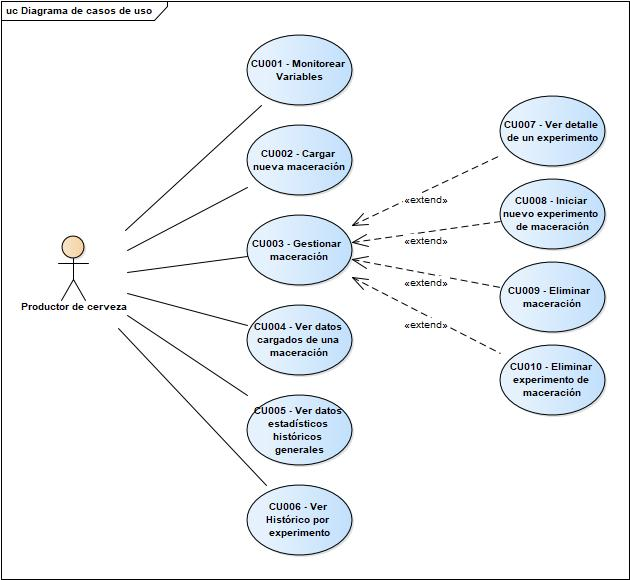
\includegraphics[scale=0.7]{DiagramadeCasosdeUso.jpg}}
    	\caption{Diagrama de casos de uso}
	    \label{DiagCU}
	\end{figure}
%	\end{minipage}
	
    
    
    
    

    